\chapter{GPGPU}

With high demand for real-time image processing, computer vision applications and a need for fast calculations in the scientific world, general-purpose computing on GPU (Graphics Processor Units), also known as the GPGPU, has become a popular programming model to accelerate programs traditionally coded on the CPU (Central Processing Unit).

Until the last decade or so, when technologies for GPGPU became available, the GPU was used mostly to render data given to it by the CPU. This has changed in a way, that the GPU, with its massive parallel capabilities, isn't used only for displaying, but also for computation. The approach to this is to transfer data bidirectionally between the CPU and the GPU, which on one hand brings the overhead of copying the data, but on the other enables to do the calculations many times faster due to the architecture of the GPU. As shown on \ref{fig:cpu-gpu} many more transistors are dedicated to data processing instead of cache or control, which leads to a higher memory bandwidth.

\begin{center}
\begin{figure}[h]
	\centering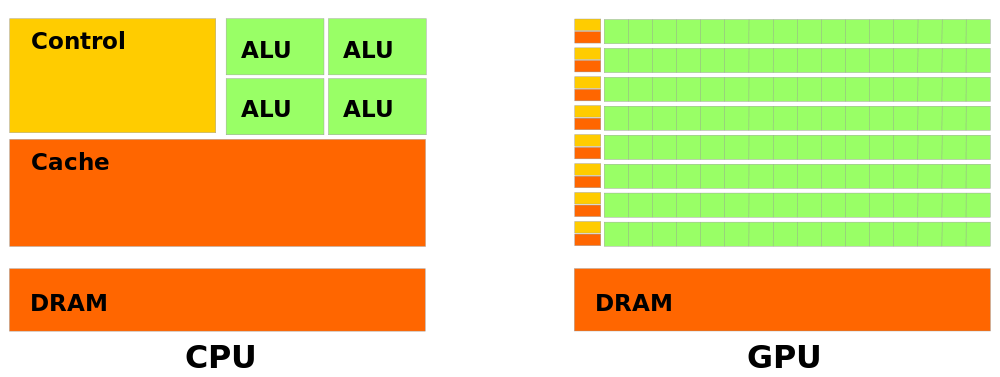
\includegraphics[height=5cm]{fig/cpu-gpu.png}
	\caption{CPU and GPU architecture comparison (\cite{cuda-toolkit-docs})}
	\label{fig:cpu-gpu}
\end{figure}
\end{center}

GPUs are also designed with floating-point calculations in mind, which can be taken advantage of, in applications such as object detection, where most of the math is done using single-precision floating-point arithmetic.

\begin{center}
\begin{figure}[h]
	\centering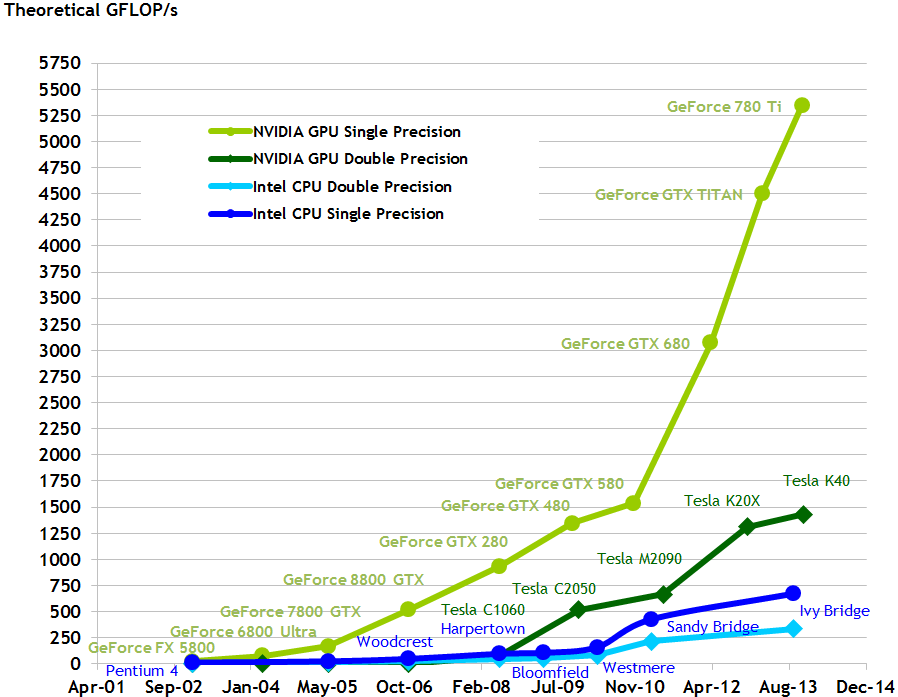
\includegraphics[height=10cm]{fig/floating-point-operations-per-second.png}
	\caption{Floating-Point operations per second for the CPU and GPU (\cite{cuda-toolkit-docs})}
\end{figure}
\end{center}

\section{Parallel computing platforms}

In November 2006 the first parallel computing platform - CUDA (Compute Unified Device Architecture) was introduced by NVIDIA. Since then the world of GPUs and computer graphics have changed significantly. The GPU stopped to be viewed only as a tool for displaying, but became another processing unit. By introducing CUDA to programmers, suddenly its programming model and memory model became available for use. 

The most widely used GPGPU platforms are the following.

\begin{itemize}
	\item CUDA - NVIDIA
	\item OpenCL - Khronos Group
	\item C++ AMP - Microsoft	
	\item Compute shaders - OpenGL
	\item DirectCompute - Microsoft
\end{itemize}

All of the technologies above allow access to the GPU computing capabilities. The first two - CUDA and OpenCL work on a kernel basis. As a programmer, you have access to low-level GPU capabilities and have to manage all the resources yourself. The standard approach is the following:

\begin{enumerate}
	\item Allocate memory on the GPU
	\item Copy data from the CPU to the allocated memory on the GPU
	\item Run a GPU based kernel (written in CUDA or OpenCL)
	\item Copy processed data back from the GPU to the CPU
\end{enumerate}

C++ AMP is a more higher-level oriented library. Introduced by Microsoft as a new C++ feature for Visual Studio 2012 with STL-like syntax, it is designed to accelerate code using massive parallelism. Currently it is supported by most GPUs, which have a DirectX 11 driver.

The last two - Compute shaders and DirectCompute also work in a more high-level fashion, but quite differently from C++ AMP. They are not a part of the rendering pipeline, but can be set to be executed together with other OpenGL or DirectX shaders.

\subsection{Evolution of the graphics pipeline}

This change towards a more general-purpose use of GPUs can be also viewed in the current OpenGL pipeline, with which most graphics programmers are familiar. In OpenGL 2.0 (2004) shader programs were introduced enabling to partially program the pipeline itself. With OpenGL 3.* (2008-2010) the shader language had improved significantly and geometry shaders were introduced. Later on in 2010 another programmable stage was introduced with OpenGL 4.0 - the tesselation shader, but still these were set stages with a predefined purpose. The most significant year for the GPGPU was 2012 with OpenGL 4.3 and the Compute Shaders. 

Compute shaders are very specific. They don't have a set number of inputs, outputs or a place in the pipeline. It is up to the programmer to specify these and also to specify a space on which they operate, like per-pixel or per-vertex basis, by fetching the data itself. This means that even the graphics pipeline, traditionally used for visualization, changed in a way, that it can be programmed without the use of traditional shaders, with compute shaders only and a more general-purpose use in mind.

\section{NVIDIA CUDA}

NVIDIA CUDA is a programming model enabling direct access to the instruction set and memory of NVIDIA GPUs. The other main competitor to CUDA, on the market, is OpenCL. Both of these models are designed with direct access to the GPU's capabilities in mind compared to other parallel platforms. OpenCL has the advantage of not being platform specific. It is supported by both major GPU vendors AMD and NVIDIA. CUDA is only usable on NVIDIA cards, but offers more options to the programmer.

\subsection{Programming model}

CUDA uses a language called CUDA C, which is an extension to C and uses NVCC compiler to generate code for the GPU. It also allows to write C-like functions called kernels. A kernel is defined by the \verb|__global__| declaration specifier and is executed using a given configuration wrapped in \verb|<<< ... >>>|. The configuration is specifies a grid and takes as parameters the number of blocks and the number of threads per block. The same kernel code is run by the whole grid. Code run by the kernel on the GPU is called the device code, whereas the code run outside of the kernel by the CPU is called the host code.

\subsubsection{Thread hierarchy}\label{subsubsec:thread-hierarchy}

\paragraph{Threads} are a basic computational unit uniquely identified by 3-dimensional indexes \verb|threadIdx| (an index within a block) and \verb|blockIdx| (an index of a block).

\paragraph{Blocks} are groups of threads, where every block resides on a single processor core, therefore a kernel can be run with the maximum of 1024 threads. Each block is uniquely identified by a 3-dimensional index \verb|blockIdx|. Threads within a block can be synchronized by a \verb|__syncthreads| call, but blocks themselves can't be synchronized, and so a new kernel must be run to do so.

The code is executed in a SIMT (Single Instruction, Multiple Thread) fashion, which is very similar to the commonly known SIMD (Single Instruction, Multiple Data) architecture. In reality the code is executed in groups of 32 threads, referred to as warps and a single Kepler or Maxwell multiprocessor supports up to 64 active warps. The important thing to mention about warps is, that when a single thread within a warp is active, the whole warp stays active and so performance-wise it is important to optimize the code to occupy warps as much as possible.

\begin{center}
\begin{figure}[h]
	\centering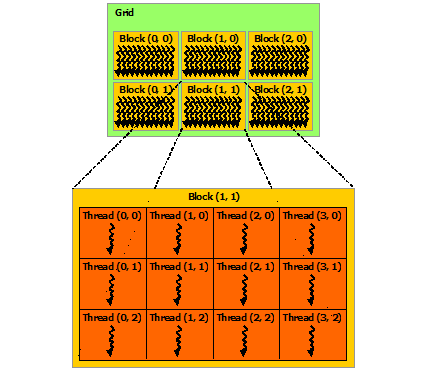
\includegraphics[height=5.5cm]{fig/grid-of-thread-blocks.png}
	\caption{A grid of blocks and threads run by a kernel (\cite{cuda-toolkit-docs})}
\end{figure}
\end{center}

Kernel configuration parameters can be passed as integers or \verb|dim3| structures. \verb|dim3| specifies the number of threads or blocks in every dimension, therefore a \verb|dim3 threadsPerBlock(4,4,1)| would run a kernel with 16 threads per block, where \verb|threadIdx.x| would range between 0 and 3 and the same for \verb|threadIdx.y|.

Example \ref{code:cuda-example} shows how to add 2 arrays in parallel using N threads and 1 block.

\begin{figure}[h]
\begin{verbatim}
// Kernel definition
__global__ void VecAdd(float* A, float* B, float* C)
{
    int i = threadIdx.x;
    C[i] = A[i] + B[i];
}

int main()
{
    ...
    // Kernel invocation with N threads
    VecAdd<<<1, N>>>(A, B, C);
    ...
}
\end{verbatim}

\caption{Example of vector addition in CUDA (\cite{cuda-toolkit-docs})}
\label{code:cuda-example}
\end{figure}

\FloatBarrier
\subsection{Memory model}\label{subsec:memory}

Another important aspect of CUDA are the types of memories, which can be used. They range from locally accessible registers with extremely fast access to globally accessible global memory, which takes hundreds of cycles to read or write to or from. They are summarized by the following table:

\begin{table}
\centering
\begin{tabular}{| l | l | l | l | l |}
\hline
Memory & Keyword & Scope & Access & Lifetime \\
\hline
Registers & - & Thread & Read/Write & Kernel \\
\hline
Local memory & - & Thread & Read/Write & Kernel \\
\hline
Shared memory & \verb|__shared__| & Block & Read/Write &  Kernel \\
\hline
Global memory & \verb|__device__| & Grid & Read/Write & Application \\
\hline
Texture memory & - & Grid & Read-only & Application \\
\hline
Constant memory & \verb|__constant__| & Grid & Read-only & Application \\
\hline
\end{tabular}
\caption{Memory types}
\end{table}

\paragraph{Global memory} is accessible by all threads in a grid and allows both read and write. It is also the slowest memory type. Its access is the bottleneck for most applications with access latency ranging from 400 to 800 cycles. There are several strategies for it to be fast like coalescing access with 32B, 64B, 128B transactions.

\paragraph{Texture memory} can be regarded similarly to global memory. Cache is optimized for 2D spatial access pattern and address modes or interpolation can be used at no additional cost.

\paragraph{Constant memory} is the third memory type, which can be accessed by all threads and is typically used to store constants or kernel arguments. It doesn't bring any speed-up compared to global or texture memory, but it is optimized for broadcast, which means that it is optimal to use it, when the same data is accessed by all the blocks.

\paragraph{Shared memory} can be accessed by all threads within a block. It is much faster than the other types, but is commonly subjected to bank conflicts. It is mainly used for acceleration, when synchronization isn't needed.

\paragraph{Unified memory} is a memory type introduced in CUDA 6.0. It enables to use the same memory addresses both in host and device code, which simplifies writing code. On the other as of spring 2014, there doesn't seem to be any hardware support \cite{unified-memory} and performance-wise the unified memory performs very similar to global memory.

\paragraph{Local memory} is a part of global memory, where everything which doesn't fit into registers is stored. For devices with Compute Capability 2.x there are 32768 32-bit registers.

\begin{center}
\begin{figure}[h]
	\centering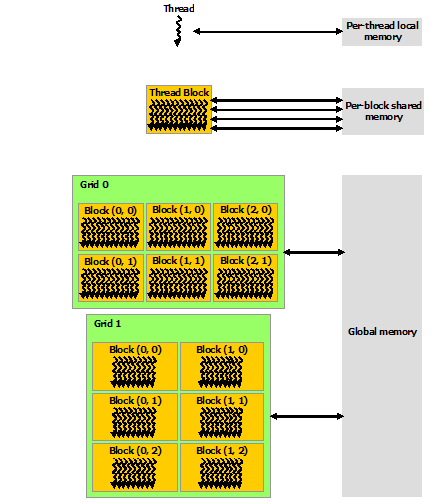
\includegraphics[height=12cm]{fig/memory-hierarchy.png}
	\caption{Memory hierarchy (\cite{cuda-toolkit-docs})}
\end{figure}
\end{center}

\subsection{Optimization methods}

\subsubsection{Global memory coalescing}

\textbf{TODO}

\subsubsection{Shared memory usage}

\textbf{TODO}

\subsubsection{Thread synchronization}

\textbf{TODO}

\chapter{Object detection}

\section{Introduction}

Object detection is a computer technology with the capability of localizing an object in input image data. The type of object depends on which data the detector was trained for. Typical applications are human faces, pedestrians, cars, traffic signs and others.

Detector used by the implementation is a frontal-face human detector, which tries to identify a human face within an image. The implementation is therefore optimized for human faces, which means, that the software can be used with other detectors, but it might effect its performance due to specific optimizations. Combined with the capabilities of a GPU, the aim is to produce an object detector capable of real-time object detection on videos or processing large amounts of images.

\section{Features}

There are several methods how to access the topic of object detection. In the following sections we will discuss feature-based object detection.

Let's take a frontal human face as an example. Despite the differences such as lighting, color of eyes or skin or the length of hair, we as humans, can identify we are looking at a human face based on similarities. For example a pair of eyes, a nose, a pair of ears and so on. These similarities can be called features, but to a computer, they are still too abstract and cannot be enumerated, and so a lot of different feature methods were devised.

\subsection{Local Binary Pattern}

One of the feature methods to describe an image are local binary patterns (LBP). They are based on encoding local intensities of an image with 8-bit codes. In their elementary form, they take a 3x3 area as an input and compare intensity values of all the pixels with the central one.

\[
 compare(p_{middle},p_{i}) =
  \begin{cases}
   1 & \text{if } p_{i} \geq p_{middle} \\
   0 & \text{else}
  \end{cases}
\]

LBP value is then evaluated as follows:

\begin{equation}
lbp(p_{middle})=\sum_{i=0}^{7} 2^{i}
compare(p_{middle},p_{i})
\end{equation}


\begin{center}
\begin{figure}[h]
	\centering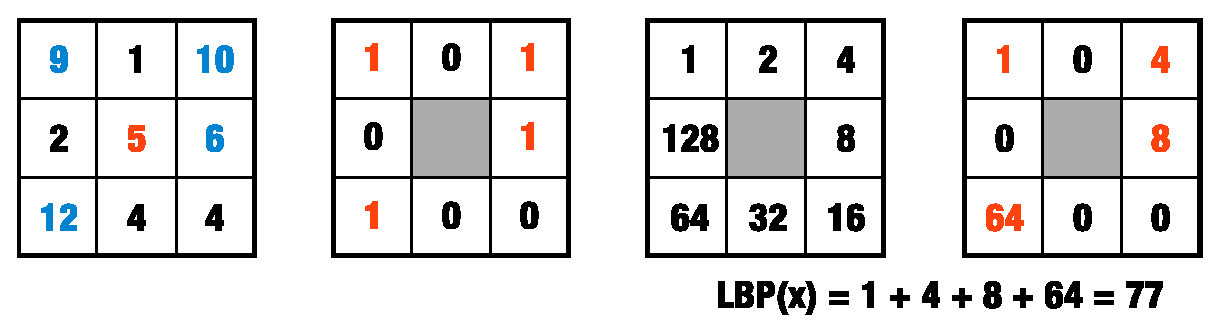
\includegraphics[width=12cm]{fig/lbp.eps}
	\caption{LBP feature}
\end{figure}
\end{center}

LBPs can be extended to be used not only for single pixels and thus 3x3 areas, but also for larger areas. When comparing larger areas, the sum of the areas is compared instead of single pixel values. For example a 2x2 LBP would sum up areas of 4 pixels and compare them with the sum in the middle.

LBP features are invariant to lighting changes, because even though the image is lighter or darker, the intensity differences stay the same. On the other hand they are not invariant to geometrical transformations such as scale or rotation.

As mentioned later on in \ref{sec:memory-organization}, the areas don't necessarily have to be summed up, but can be interpolated instead, because the LBP code generated after comparing average values and summed up values is the same.

\section{Waldboost}
\label{sec:waldboost}

Each LBP feature represents a single weak classifier, which decides whether the given sample corresponds to the sought object or not. On the other hand only one feature cannot describe the whole face, so a meta-algorithm to process a series of such weak classifiers is needed, combining them in a single strong classifier.

One such algorithm is WaldBoost, which combines AdaBoost and Wald's Sequential Propability Ratio Test (SPRT). SPRT is a strategy to determine what class a sample belongs to, based on a series of measurements.

\[
 SPRT =
  \begin{cases}
   +1 & \text{if } R_{m} \leq B \\
   -1 & \text{if } R_{m} \geq A \\
   \# & \text{else take another measurement} 
  \end{cases}
\]

$R_{m}$ is the likelihood ratio and A, B are constants to compute the wanted false negatives $\alpha$ and false positives $\beta$ ratios as follows:

\begin{equation}
R_{m}=\frac{p(x_{1}, ..., x_{m}|y=-1)}{p(x_{1}, ..., x_{m}|y=+1)}
\end{equation}

\begin{equation}
A=\frac{1-\beta}{\alpha}, B=\frac{\beta}{1-\alpha}
\end{equation}

As mentioned in \cite{sochman-matas-waldboost} with face detection in mind, the positive rate $\beta$ can be set to 0 and the required false negative rate $\alpha$ to a small constant. As such the equations can be simplified to

\begin{equation}
A=\frac{1-0}{\alpha}=\frac{1}{\alpha}, B=\frac{0}{1-\alpha}=0
\end{equation}

and the whole strategy to

\[
 SPRT =
  \begin{cases}
   +1 & \text{if } R_{m} \leq 0 \\
   -1 & \text{if } R_{m} \geq \frac{1}{\alpha} \\
   \# & \text{else take another measurement} 
  \end{cases}
\]

$R_{m}$ is always positive and therefore the algorithm will only classify the sample as a face when it finishes its training cycle or discard it as a background when the ratio gets greater than the given constant A.

\chapter{Analysis}

The idea of implementing a WaldBoost object detector with the use of LBP features on a parallel platform is not a new one. On the other hand, since it was first proposed, both OpenCL and CUDA have undergone many changes and as such optimizations and different approaches to the implementation can be discussed.

The implementation of a WaldBoost detector on a CPU, where every pixel is processed sequentially isn't complicated. The general idea, as explained in \ref{sec:waldboost}, is that a sample, in our case a pixel, is processed by a series of weak classifiers, in the implementation called stages. These stages accumulate a response, always adding or subtracting a value based on how the LBP feature is evaluated. In case the accumulated response gets greater than a certain value, the sample is discarded, the program skips the rest of the classifiers and continues with the next pixel.

Image processing tasks are generally suitable for parallel acceleration. On the other hand it is not as simple. The number of pixels is huge and as shown in \ref{fig:survivors}, most of the samples get discarded as background after few initial stages. On a parallel platform, such as the GPU, this presents a problem, because most of the processors have to wait for the few samples, that are still being processed and thus wasting a lot of resources.

\begin{center}
\begin{figure}[h]
	\centering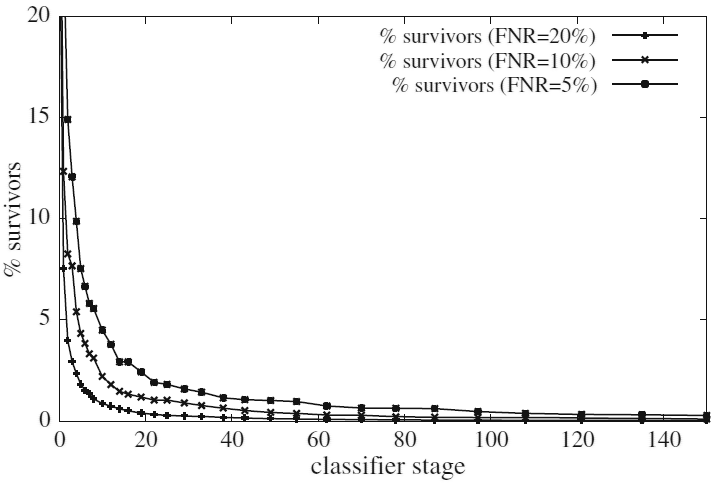
\includegraphics[width=0.6\linewidth]{fig/survivors.png}
	\caption{Surviving percentage of samples gets below 5\% after few initial stages. Taken from \cite{herout-realtime-cuda}.}
	\label{fig:survivors}
\end{figure}
\end{center}

\section{Real-time object detection on CUDA by Herout et al., 2009}

Most of the current implementations of WaldBoost detectors are based on this work. As mentioned previously and shown in \ref{fig:survivors}, only a few samples are being processed after few initial stages. The rest of the samples still occupy GPU resources and wait for these to finish. To free these resources and use them accordingly, a method of thread rearrangement was proposed.

\subsection{Pyramidal image}

The detector uses a window for scanning the image, usually 24x24 or 26x26 pixels. In order to detect the object in such window, a pyramidal image was proposed. Such image contains many sub-sampled images stored in a pyramid fashion. The implementation details are discussed in \ref{subsec:pyramidal}.

\subsection{Thread rearrangement}

At the time of writing the paper, detectors with 512 or 1024 stages were used (our implementation uses a detector with 2048 stages). Herout et al. proposed, that every sample can be processed up to a set number of stages, after which thread rearrangement is done as described in \ref{fig:thread-rearrangement} and the process continues.

\begin{center}
\begin{figure}[h]
	\centering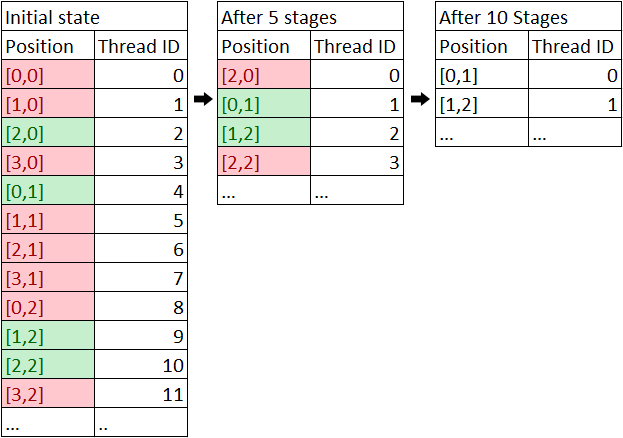
\includegraphics[width=0.6\linewidth]{fig/threadrear.png}
	\caption{Thread rearrangement of surviving threads (green) after 5 and 10 processed stages.}
	\label{fig:thread-rearrangement}
\end{figure}
\end{center}

Methods how to achieve this rearrangement are again specific to the implementation and are discussed later in \ref{subsec:thread-reorganization}.

\chapter{Implementation}

The object detector is implemented in C++ with dependencies on OpenCV\footnote{\url{http://www.opencv.org}} - an open source computer vision library with C and C++ interfaces and CUDA\footnote{\url{http://www.nvidia.com/object/cuda_home_new.html}} - a library for writing NVIDIA GPU code with a CUDA C interface, which is an extension to C compiled by the NVCC compiler.

It is implemented as an easy-to-use class, which takes a dataset or a video on the input and outputs detections. As such, it can be used as a part of an application such as face tracking or face recognition, but not only faces have to be processed, depending on what the detector is trained on.

\begin{center}
\begin{figure}[h]
	\centering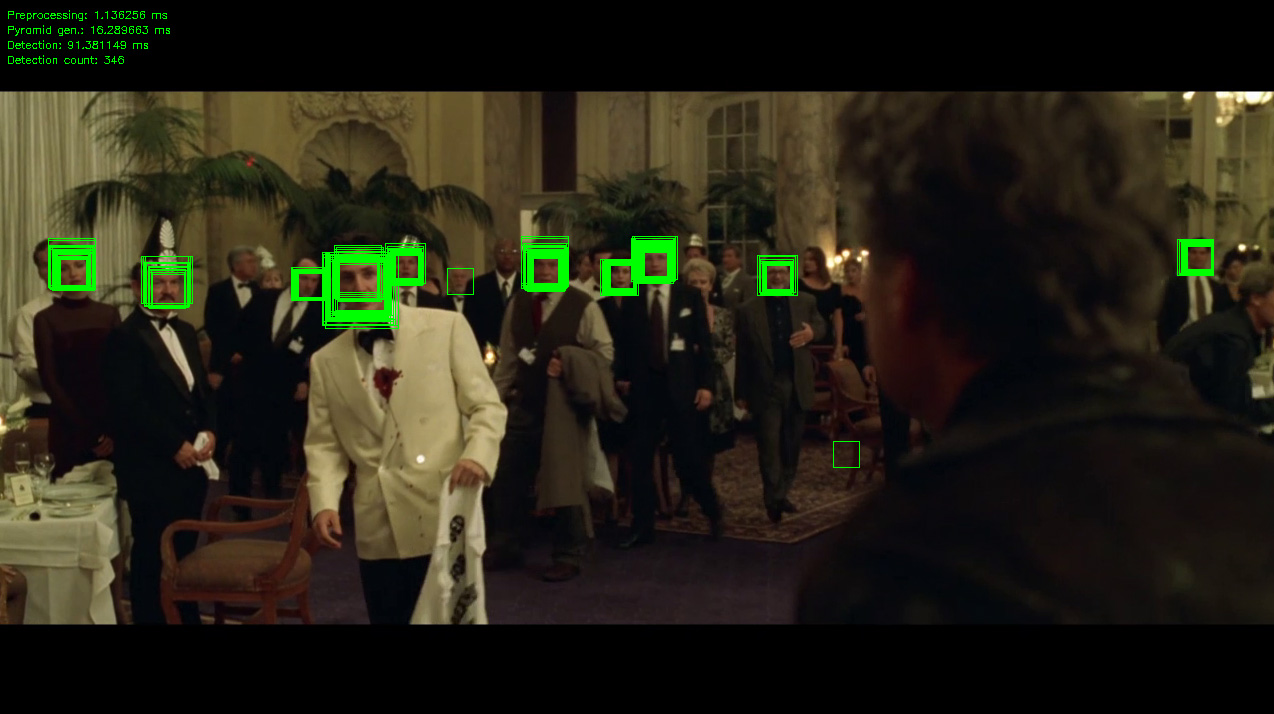
\includegraphics[width=0.8\textwidth]{fig/sample.jpg}
	\caption{A sample output with a lot of detections around each object}
	\label{fig:sample}
\end{figure}
\end{center}

\section{Face tracking and recognition}

A previous version of the current implementation was already used as a part of a project for face tracking and recognition on a video, which might be a typical use case for security cameras.

In order to track a face, the face has to be recognized in previous frames, as such for every processed frame, all the faces have to be detected. The detector processes the frame and outputs detections. The detections are then processed as follows:

\begin{enumerate}
	\item \textbf{Choose the best response detection.} There are usually more detections for every face, depending on the number of sub-sampled images. Out of the overlapping detections, the detection with the best response is chosen.
	\item \textbf{Coversion to HSV.} The detection (a square-sized area) is converted to HSV (Hue, Saturation, Value color model) and a histogram is calculated. For a human face, the V component can be dropped, which provides luminance invariability.
	\item \textbf{Histogram comparison.} The histogram of H and S values is compared with the histogram of all the previously found faces. The distance from the detection is also taken into consideration, because we presume the face doesn't change positions too much.
\end{enumerate}

To calculate the difference between two ROI historgram different methods can be used. In this case Bhattacharyya distance \ref{eq:bhatta}.

\begin{figure}
\begin{equation}
d(H_{1},H_{2})=\sqrt{1-\frac{1}{\sqrt{\overline{H_{1}}\overline{H_{2}}N^2}}\sum\limits_{I}\sqrt{H_{1}(I) \cdot H_{2}(I)}}
\end{equation}
\caption{Bhattacharyya distance}
\label{eq:bhatta}
\end{figure}

In order to track or recognize a face in real-time, both the detection and the recognition have to be processed faster, than the framerate.

\section{Detector}

The detector can be used to detect any object it is trained to, not only faces. Most detectors are stored as XML files, which brings the overhead of reading and parsing a file. Because of that the detector is passed as 2 header files (\verb|wbd_detector.h|, \verb|wbd_alphas.h|) and compiled with the detector.

These headers can be obtained by parsing a XML detector \footnote{\url{https://github.com/mmaci/classifier-export}}. The detector consists of two main parts, the stages or also called the weak classifiers, which are loaded into a structure \ref{fig:stage} and an $\alpha$-table, which is stored as an array if floating-point values. Every stage points to a specific range inside the $\alpha$-table, where responses for all the LBP values are stored. Training of a detector is not the subject of this thesis and as such it will not be discussed.

\begin{figure}[h!]
\begin{verbatim}
struct Stage {
    uint8 x, y; // X, Y offsets
    uint8 width, height; // width, height of the feature
    float thetaB; // threshold
    uint32 alphaOffset; // alpha table offset
};
\end{verbatim}
\caption{Stage structure}
\label{fig:stage}
\end{figure}

\section{WaldboostDetector class}

The WaldboostDetector class is designed to simplify the detection as much as possible. It can be used only by loading a video or a dataset and then running the \verb|run()| method, which returns a list of detections. Optionally the programmer can set specific settings described in \ref{sec:options}. On the other hand when not set, these are set optimally based on results obtained by measurements on different GPUs.

\section{Program cycle of WaldboostDetector}

The detector processes both videos and image datasets, which are passed to the detector as a filename. For the dataset a text file is used with filenames of the images separated by a newline. OpenCV is used to load both images and videos and as such it supports most common formats.

The application pipeline (\ref{fig:pipeline}) of the detector is a bit different for a dataset, than for a video, but both use the following steps as described in \ref{subsec:init} to \ref{subsec:free}.

\begin{center}
\begin{figure}[h!]
	\centering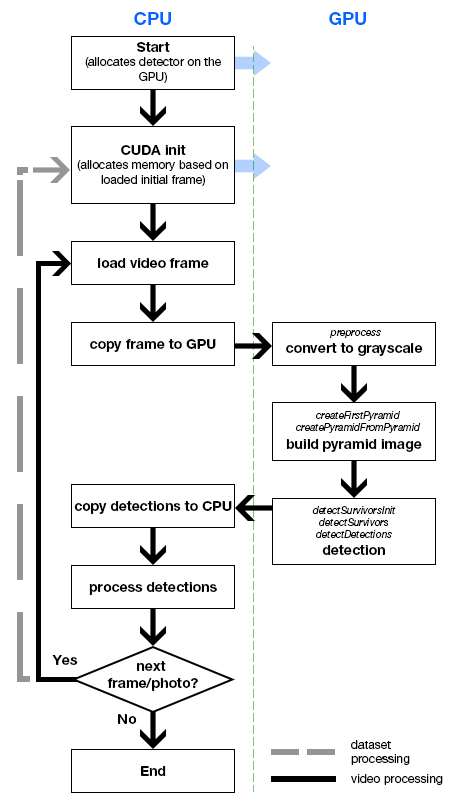
\includegraphics[width=9cm]{fig/pipeline.png}
	\caption{Application pipeline. On the GPU side, kernel methods are mentioned.}
	\label{fig:pipeline}	
\end{figure}
\end{center}

For a video, the detector can be initialized only once with the initial frame. All the other frames have the same size and so the same memory structures can be used. Image setup and the Detection are then run multiple times for every frame. After the video is processed, memory is freed.

For a dataset, every image can be different and so the whole process must be run multiple times for every loaded image.

A CMake project is included, therefore it can be built on multiple platforms. As for the project itself, it is logically separated into the following modules and sub-modules (in code this is done using C++ namespaces):

\begin{itemize}
	\item simple - a simple C++ implementation without any optimizations
	\item gpu - a GPU implementation using CUDA
	\begin{itemize}
		\item pyramid - pyramidal image generation
		\item detection - detection processing
	\end{itemize}
	\item WaldboostDetector - a class for simple handling
\end{itemize}

\subsection{Initialization}\label{subsec:init}

The initialization of the detector can be separated into two parts. The first being the tasks, that have to be done only once for both datasets and videos. This means copying the detector into GPU memory (the detector contains weak classifiers/stages and an $\alpha$-table). This is done in the constructor of the WaldboostDetector class.

The other part being allocating GPU memory for the image itself, which is allocated dynamically due to dependence on the size of the input image. For a video this can also be done only once, because every frame has the same size and as such, everything is allocated based on the initial frame. On the other hand a dataset can have completely different image sizes and so this must be done for every photo separately.

A method to skip multiple initialization for datasets was proposed by allocating a single large texture, which can be a solution, but leads to questions, such as what do we mean by a large enough texture.

\subsection{Setting an image}

After the initialization is complete, an image or a frame is loaded by OpenCV and then copied over to the GPU. This must be done both for every image or every frame. It resides only in a chunk of global memory. It is set as a texture later on, after preprocessing \ref{subsubsec:grayscale}.

\subsection{GPU Kernels and detection}

After initializing the detector, memory structures and copying the image, everything is set to run the detection process, which consists of several parts:

\begin{itemize}
	\item Preprocessing
	\item Creating a pyramidal image
	\item Detection
\end{itemize}

\subsubsection{Preprocessing} \label{subsubsec:grayscale} 

First the initial loaded image has to be preprocessed. There are 2 operations to be done - conversion from the initial integers to a floating-point representation and then a conversion to grayscale.

Floats are needed in order to work with textures. Texture memory enables hardware implemented bilinear interpolation for subsampling images, which is done mainly in creating the pyramidal image (\ref{subsubsec:pyramidal}. Even though bilinear interpolation should only be supported for floating-point values, due to official documentation, it is not the case. On the other hand it might be a bug, which might get fixed in the future and it would be wise not to be used.

Conversion to grayscale is a simple image processing operation described by the formula \eqref{eq:rgbtograyscale}. The detector itself is trained on grayscale images, and so the input must also be in grayscale. After the kernel finishes, the result is saved as a texture.

\begin{equation} \label{eq:rgbtograyscale}
Y=0.2126R + 0.7152G + 0.0722B
\end{equation}

\subsubsection{Dynamic texture and texture objects}

As of CUDA 5.0 and Kepler GPUs textures don't have to be defined globally as static textures, but they can be used dynamically using Texture Objects (\verb|cudaTextureObject_t| class API \cite{cuda-texture-obj}).

This has several advantages. One of them being the slight overhead (up to 1.5 \mu s) by binding and unbinding static textures during kernel launch, which is eliminated. Even though this is not our case and doesn't sound as much, it might be quite a significant overhead while launching large quantities of fast kernels.

The main advantage in our case is, that texture objects can be passed as arguments, set to store variable image sizes and therefore easily be used as a part of a library. Also multiple textures can be created using given parameters, which is exploited in pyramidal image creation and explained in \ref{subsec:pyramidal}.

\subsubsection{Pyramidal image}\label{subsec:pyramidal}

All the pixels are processed using a 26x26 pixel-wide window. The size again depends on how the detector is trained. The basic idea is that for the given object, all the features describing it fit inside this window. On the other hand objects, such as faces, are usually much larger in the initial image, therefore we have to create many sub-sampled images and run the detection on every one of them.

In order to do this, the straight forward method is to create a pyramidal image and store it as a texture on which the detection is run.

As mentioned previously, the implementation uses hardware bilinear interpolation provided by the texture memory for sub-sampling the image. It has to be kept in mind, that bilinear interpolation has some negative side-effects, one of them being the sub-sampling of an image below half its original width.

\begin{center}
\begin{figure}[h]
	\centering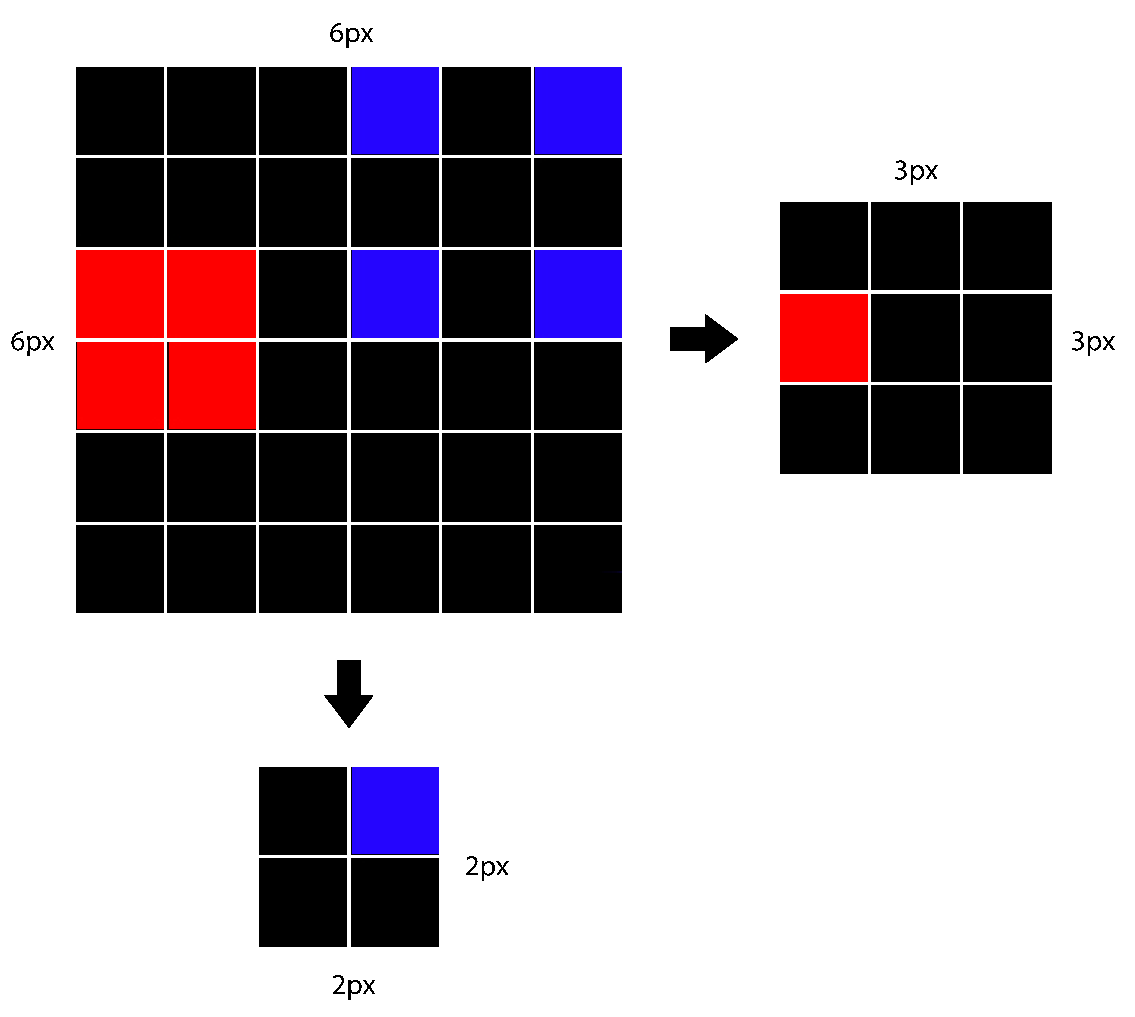
\includegraphics[height=9cm]{fig/bilinear_error.pdf}\label{fig:bilinear-error}
	\caption{Error when sub-sampling an image below twice the original width using bilinear interpolation}
\end{figure}
\end{center}

As shown on \ref{fig:bilinear-error} when sub-sampling an image below half its original width, pixels are left out and a sampling error is created. Other methods such as Lanczos %todo

The image is generated in octaves. An octave is a structure of several images, where the smallest image has half the width/height of the original image. Depending on the number of images in an octave, every image is $2^1/number_of_images$ smaller than the previous. The following octave is then sub-sampled from the previous octave.

Two methods were tested. The first one using a single texture for both writing a reading the individual octaves. This proved to be very costly and therefore another method had been implemented and is described below:

\begin{enumerate}
	\item A pyramidal image of $N$ images is generated, where each image is $2^1/N$ smaller then the previous. Every image is sub-sampled from the original image.
	\item Generated pyramidal image is stored as a dynamic texture. Simultaneously the pyramid is being written inside a final image used for detection.
	\item A pyramidal image is generated, by sub-sampling the previously generated pyramid. Width and height of the sub-sampled pyramid are twice smaller than that of the original.
	\item Generated pyramidal image is saved as a dynamic texture.
	\item Steps 3 and 4 get repeated for a set number of octaves.
\end{enumerate}

\begin{center}
\begin{figure}[h]
	\centering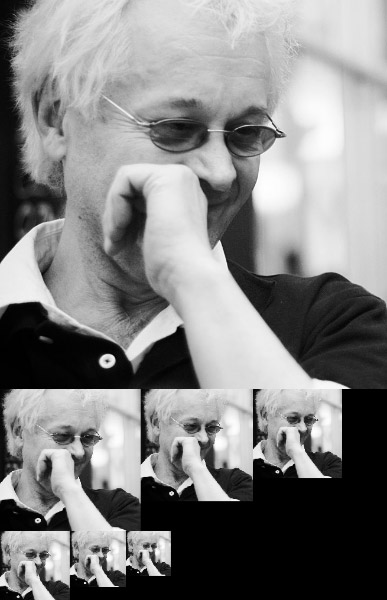
\includegraphics[height=9cm]{fig/pyramid.jpg}
	\caption{Pyramidal image}
\end{figure}
\end{center}

The implementation itself uses 8 levels and 4 octaves. This results in the sides of the smallest image being 16x smaller than the original. By reducing the number of octaves or levels, better performance can be gained, but it will be get reflected in the number of detections.

\subsubsection{Detection}

A Waldboost detector consists of several parts. First we will discuss the general idea of a waldboost detector and the memory organization of the different structures. Then we will focus more on the details of the implementation.

\begin{itemize}
	\item $\alpha$ coefficient table
	\item stages
	\item final threshold
\end{itemize}

To detect an object, the detector has to successfully evaluate a given number of stages (weak classifiers), which are processed sequentially. In our case 2048. This number can be reduced, but it will have an impact on the number of detections. Every stage the algorithm processes, a response is given by the $\alpha$-table, where position is the stage's $\alpha$-offset and the calculated LBP value. It is then added to the accumulated response. The sample is discarded in case the accumulated value falls below the threshold \verb|thetaB|.



The detector uses a 26x26 pixel-wide window, where \verb|x| and \verb|y| are offsets inside the window and \verb|width| and \verb|height| describe the size of the feature. \verb|alphaOffset| is an offset inside the $\alpha$-table corresponding to appropriate LBP values. \verb|thetaB| is the threshold value, which decides if the sample gets discarded or not in the current stage.

\begin{algorithm} \label{alg:detection}
\For{every pixel (a GPU thread is created)}
{
	\For{every stage}
	{
		1. compute LBP coefficient \\
		2. add response for the given LBP to the accumulated response \\
		\If{accumulated response $\geq$ stage threshold $thetaB$}{
			discard sample
		}
	}
}

\caption{Object detection algorithm simplified}
\end{algorithm}

\subsection{Freeing the memory}

After everything has been processed, the GPU memory can be freed. This also must be done for every image in case of a dataset, but only once in case of a video.

\section{Memory organization} \label{sec:memory-organization}

The use of GPU memory is one of the most important parts of programming on GPU architectures. The types of CUDA memories are described in \ref{subsec:memory}.

Below we will discuss, how the most important parts of the detector are stored and why.

\begin{itemize}
\item \textbf{Stages/Weak classifiers} - constant memory \\
Stages are stored in the constant memory. Even though it's not as fast as let's say shared memory, its capability to broadcast simultaneously accessed data is ideal. Every thread processes a single image position, for which it loops through a for-cycle of stages. Every read from the constant memory is then not only broadcast to a half-warp (a group of 16 threads), but also cached. The only problem can be the size, which is limited to 64 KB. The detector uses 2048 stages, where each stage is 12 B. This leads to 24 KB, which is enough, but has to be accounted for when storing other data in the constant memory.

\item \textbf{$\alpha$-table} - texture memory \\
There are 256 coefficients for every stage and every coefficient is stored as a float. This leads to $256 * 2048 * 4 = 2 MB$ and by far exceeds the memory available for constant memory. Another reason the constant memory cannot be used is that the access is random, due to the fact, that we are likely to get different LBP values for every pixel. In this case we wouldn't utilize the broadcast and it would even be slower.

\item \textbf{Original image and pyramidal image} - texture memory \\
Both are stored in the texture memory. Original image is used to create a pyramidal image using hardware accelerated bilinear interpolation for creating down-sampled images as described in \ref{subsec:pyramidal}. It is highly optimized for random read-only access, which is exactly what we want.
\end{itemize}

\section{Thread allocation}

A GPU thread is allocated for every sample, therefore every pixel. Based on \cite{herout-realtime-cuda} only a fraction of samples (around 1\%) is still processed by the classifier after only 10 stages. On the other hand the GPU organizes threads in warps - groups of 32 threads, which are organized in blocks across with they can be synchronized. The problem is that, when only a single thread within a warp is active, the other threads have to wait for it until it finishes thus wasting GPU resources.

\cite{herout-realtime-cuda} proposed, that every few stages threads can be checked if they are still evaluating the classifier stages or they have been dropped. Surviving threads can then be reorganized to continue within fewer warps and the other resources to be freed.

\section{Thread reorganization}\label{subsec:thread-reorganization}

The detector uses several ways of reorganizing surviving threads. They are summarized below by the types of functions they use and where surviving threads are stored:

\begin{itemize}
	\item atomic functions / global memory
	\item atomic functions / shared memory
	\item atomic functions / hybrid global-shared
	\item prefix sum / global memory
\end{itemize}

It also uses 3 functions, which are implemented as functions within a kernel or kernel functions on their own. This depends whether the kernel can by synchronized without having to run it again.

\begin{itemize}
	\item \verb|detectSurvivorsInit| - processes all samples for a given number of stages and outputs the surviving threads. Called at the beginning.
	\item \verb|detectSurvivors| - processes surviving samples for a given number of stages and outputs the surviving threads. Called multiple times.
	\item \verb|detectDetections| - processes remaining surviving threads and outputs detections. Called at the end.
\end{itemize}

\subsection{Atomic functions and global memory} \label{subsec:afgm}

The first proposed method uses a counter stored in global memory to count the number of surviving threads within a block and global memory for storing the surviving sample information. After processing a given number of stages of a classifier, every sample which wasn't discarded by the classifier is assigned an ID in global memory based on the value of the global counter and atomically incrementing it. It then saves the information about the sample (\ref{fig:survivordata}) to global memory with the ID as an index.

\begin{figure}[h!] \label{fig:survivordata}
\begin{verbatim}
struct SurvivorData {
    uint32 x, y; // X, Y coordinates of the sample
    float response; // current response
};
\end{verbatim}
\caption{Stage structure}
\end{figure}

Threads cannot be synchronized across the whole grid (between all the threads), only across a block, therefore a new kernel must be launched. Functions themselves are implemented as kernels.

\subsection{Atomic functions and shared memory}

The global memory method has two logical downsides. One being the use of a global memory counter, which might become a serious bottleneck on an image with lots of detections. The other being the synchronization, when a whole new kernel has to be run.

To solve these issues a method exploiting the use of shared memory was proposed. All the survivors are stored in shared memory and so is the counter, which only counts surviving threads within a block.

Threads can be synchronized within a block and so the functions are not implemented as kernels like in the previous case, but only as \verb|__device__| functions. The kernel doesn't have to be run again,  in this case.

After processing a given number of classifier stages the surviving sample is assigned an ID within its block based on the value of the shared memory counter and atomically increments it. Threads are then synchronized and only the ones having ID smaller than the value of the counter continue.

\subsubsection{Advantages of the shared memory approach}

\begin{itemize}
	\item Shared memory is much faster than global memory (the bandwidth of shared memory is ~1.7TB/s compared to that of global memory which is ~150GB/s.
	\item Counters and atomic increments are distributed across shared memory removing the single counter bottleneck.
	\item Only a single kernel can be run with the use of \verb|__syncthreads| to synchronize threads inside a block every given stage.
\end{itemize}

\subsubsection{Disadvantages of the shared memory approach}

\begin{itemize}
	\item More warps are being run due to threads being packed at the start of the shared memory.
	\item An overhead of syncing threads, resetting the counter and checking for surviving threads is added.
\end{itemize}

For example if there would be only 32 surviving threads, the global memory method would only need a single warp. On the other hand the shared memory variant would probably need more warps, because the surviving threads would be distributed across more blocks.

The overhead of rerunning a kernel is quite low and so a third method was proposed.

\section{Hybrid method using both shared and global memory}

The hybrid method removes the global memory counter bottleneck and still preserves the efficiency of organizing survivors in global memory. Like in the shared memory implementation, it uses a counter stored in shared memory. Each surviving thread is assigned an ID based on this counter, after which the threads are synchronized. An offset in global memory is also stored. The current value of the offset is stored by the thread and the value of the counter is atomically added to it. The stored value is then used as an index of survivor information in global memory (\verb|shared memory ID + global memory offset|). Because an atomic add is used, in case another block wants to save its survivors, it already uses the new offset value and again atomically adds its counter.

The disadvantage is a slight overhead, where all threads inside the block have to be synchronized before the counter can be added to the offset and so all threads must wait in case any of them survives. Also both an atomic increment and an atomic add are used.

\section{Prefix-sum}

The last proposed method tries to remove the use of a counter altogether and thus removing a possible bottleneck. A parallel prefix-sum is an algorithm commonly used for such tasks. It allows to sum up values on a parallel architecture with a logarithmic complexity.

The main idea behind is, that it produces an array of values, where every element is the sum of the previous values. For an array of 0's and 1's, where 1 is a surviving thread and 0 is a discarded thread, it not sums up all the survivors in the last element, but also assigns a unique id for every thread. This is done using shared memory, where the size of the memory is the same as the number of threads in a block.

The algorithm can be viewed as a tree and be represented as an array in shared memory. It consists of two phases an up-sweep phase and a down-sweep phase. The tree is a binary tree with the values (in our case 1's and 0's) as leaves.

In the up-sweep phase, the tree is traversed from its leaves to the root, where in every stage the values are summed up in their parent as shown in \ref{fig:sweepup}.

\begin{center}
\begin{figure}[h]
	\centering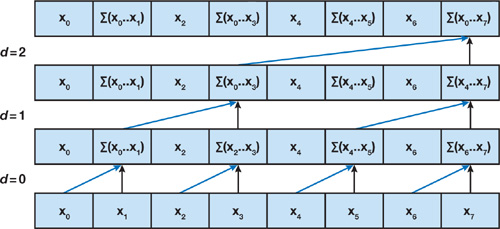
\includegraphics[width=0.6\linewidth]{fig/sweepup.jpg}
	\caption{Up-sweep phase of the prefix sum algorithm (taken from \cite{prefixsum})}
	\label{fig:sweepup}
\end{figure}
\end{center}

At the beginning half of the threads in a block are used to calculate the corresponding sums. The next iteration the number of threads used is halved and so on, until the root is reached, in which the total sum of all the values is stored.

In the down-sweep phase as shown in \ref{fig:sweepdown}, the root is zeroed and traversed back to the leaves. Using the partial sums a sum of all the previous values for every leaf is gained.

Every surviving thread is then assigned an ID based on its value in the prefix-sum array and the total number of surviving threads inside the block is the last value inside the array.

\begin{center}
\begin{figure}[h]
	\centering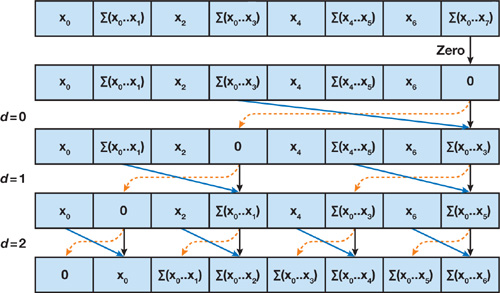
\includegraphics[width=0.6\linewidth]{fig/sweepdown.jpg}
	\caption{Down-sweep phase of the prefix sum algorithm (taken from \cite{prefixsum})}
	\label{fig:sweepdown}
\end{figure}
\end{center}

\section{Setting the thread-reorganization stages}

Thread reorganization is a costly process, but greatly enhances the performance, therefore a balance between reorganizing threads and running the detection has to be found. As described thoroughly in \ref{subsec:thread-reorganization}, every detection function call has a starting stage and an ending stage. For the initial function call, the stating stage is set to 0 and for the final stage as the number of stages - in our case 2048. It is then quite important to set these, because it will have large impact on the overall performance.

The proposed strategy is to reorganize threads every time the number of surviving threads is half the function started with. In case of the methods using global memory, this is quite unthinkable to do performance-wise. The kernel would have to be run for every stage and the number of surviving threads measured. For the shared-only memory implementation, this would be easier, as the image is processed in blocks and only a shared counter would be used. On the other it would still add a large overhead of atomically decrementing a counter and reading from it.

What we have done is, that these inefficient kernels were programmed and measured on different GPUs and as a result predefined stages were determined. The results are different based on a GPU and the type of an image, such as if there are lots of people on the images or only a few.

The detector then sets the predefined thread-reorganization stages based on the GPU used and the expected type of the scene.

\chapter{Performance measurements and profiling}

This chapter evaluates performance results obtained by measurements on different GPUs and discusses them based on results obtained from profiling. The following GPUs were used:

\begin{itemize}
	\item NVidia GeForce GTX 980
	\item NVidia GeForce GTX 780Ti
	\item NVidia Quadro K1000M
\end{itemize}

The technology used in the implementation  is supported only by Kepler architecture and newer (CUDA 5.0+). Because of this the cutting edge Kepler and Maxwell GPUs were chosen (GTX 980 for the Maxwell architecture and GTX 780Ti for the Kepler architecture) to test the limits of the implementation. Also an average notebook GPU (Quadro K1000M) was chosen to test the performance in more standard user conditions. Specifications of the GPU's can be found in \ref{tab:parameters-gpu}. The driver version used was 340.62 and for the CPU Intel(R) Core(TM) i7-3610QM CPU @ 2.30 GHz.

The tested use cases were the following:

\begin{itemize}
	\item 720x480 video
	\item 1280x720 video
	\item 1920x1080 video
	\item BioID face dataset with 1512 grayscale images
\end{itemize}

As a video a part of the movie "The Game" (1997) was used with ~10-50 faces at a time.

\begin{center}
\begin{table}[htbp]
\begin{tabularx}{\textwidth}{| X | X | X | X |}
\hline
- & NVidia GeForce GTX 980 & NVidia GeForce GTX 780Ti & NVidia Quadro K1000M \\
\hline
Architecture & Maxwell & Kepler & Kepler \\
\hline
SM's\footnote{Streaming multiprocessors} & 16 & 15 & 1 \\
\hline
CUDA Cores\footnote{Depends on the architecture. Maxwell has 128 CUDA cores per SM, whereas Kepler has 192 CUDA cores.} & 2048 & 2880 & 192 \\
\hline
Base Clock (MHz) & 1126 & 875 & 850 \\
\hline
Memory (MB) & 4096 & 3072 & 2048 \\
\hline
Memory bandwidth (GB/s) & 224 & 336 & 28.8 \\
\hline
\end{tabularx}
\caption{Parameters of graphics cards used for performance measurements}
\label{tab:parameters-gpu}
\end{table}
\end{center}

Another important thing to mention is the Compute Capabilities the object detector is targeted are 3.0 for the Kepler architecture cards and 5.0 for the Maxwell architecture GeForce GTX 980. The limits of the architectures are summarized in \ref{tab:capability-3050}. Most of the measurements discussed in \ref{sec:detection-time} will depend on these limits and so it is important to take them into consideration.

\begin{table}[htbp]
\begin{center}
\begin{tabularx}{0.75\textwidth}{| X | X | X |}
\hline
Compute Capability & 3.0 & 5.0 \\
\hline
Max. number of blocks per SM & 16 & 32 \\
\hline
Max. number of warps per SM & 64 & 64 \\
\hline
Max. number of threads per SM & 2048 & 2048\\
\hline
Max. number of threads per block & 1024 & 1024\\
\hline
Local memory per thread & 512 KB & 512 KB \\
\hline
Max. shared memory per SM & 48 KB & 64 KB\\
\hline
\end{tabularx}
\end{center}
\caption{Limits of devices for Compute Capability 3.0 and 5.0 (Maxwell)}
\label{tab:capability-3050}
\end{table}

\section{Detection time}\label{sec:detection-time}

In order for the detector to be a real-time object detector, it must process the video in under $1/framerate$ seconds. Therefore, the main focus of the measurements was on the detection time of the individual kernels.

As mentioned in \ref{subsubsec:thread-hierarchy} the kernels are initialized with a thread configuration, which can be 1D, 2D or 3D. In our case the following 2D configurations were used: 8x8 (64 threads per block), 16x16 (256 threads per block), 32x32 (1024 threads per block). The most important things, that depend on the size of a block are the size of the shared memory and the number of threads, which are synchronized using the \verb|__syncthreads| call. Only $2^N$ sizes of the blocks were tested, because specifically the prefix-sum implementation works only for those.

\begin{center}
\begin{figure}[h]
	\centering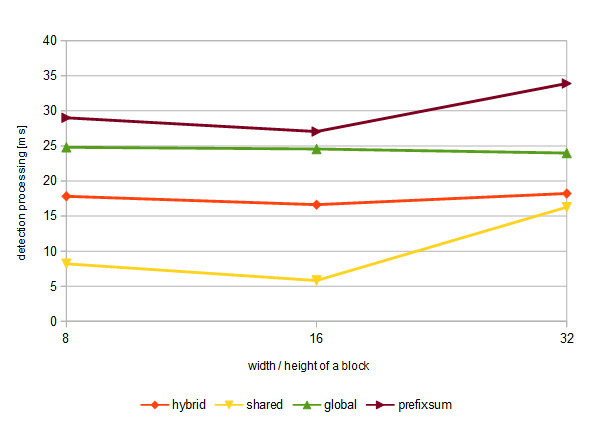
\includegraphics[width=0.85\textwidth]{fig/1080_detection_maxwell.png}\label{fig:980-det-measurement}
	\caption{Comparison of detection times of different implementations on GeForce GTX 980 (Maxwell)}
\end{figure}
\end{center}

\begin{center}
\begin{figure}[h]
	\centering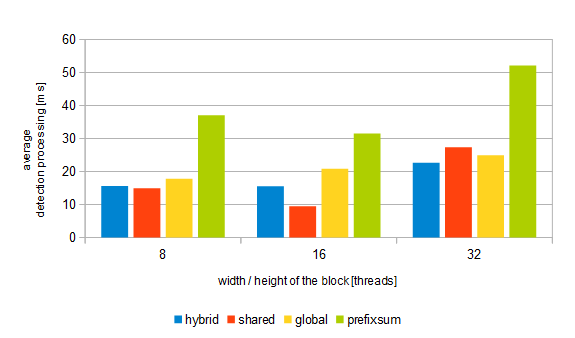
\includegraphics[width=0.85\textwidth]{fig/1080_detection_kepler.png}\label{fig:780ti-det-measurement}
	\caption{Comparison of detection times of different implementations on GeForce GTX 780Ti (Kepler)}
\end{figure}
\end{center}

\begin{center}
\begin{figure}[h]
	\centering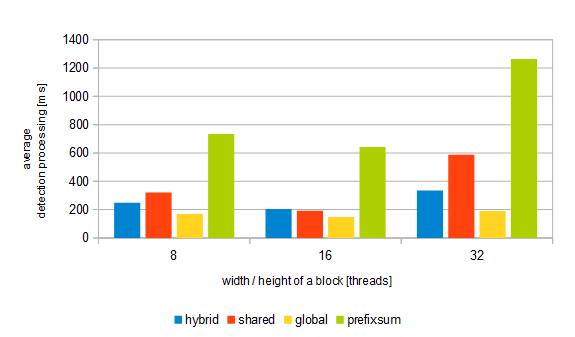
\includegraphics[width=0.85\textwidth]{fig/1080_detection_quadrok1000m.png}\label{fig:quadro-det-measurement}
	\caption{Comparison of detection times of different implementations on Quadro K1000M (Kepler)}
\end{figure}
\end{center}

\subsection{Shared and global memory}

The most interesting thing to note is that, for the Quadro K1000M the fastest implementation is actually the global memory implementation, because the memory access doesn't seem to be the bottleneck here, but the calculation itself. This can also be seen for the hybrid and shared implementations, where it was assumed, that the global counter would cause a decrease in performance. It did on the other GPU's, but in case of Quadro K1000M, the card seemed more affected by the computational overhead of the algorithm.

\subsection{Prefix-sum}

The prefix-sum implementation performed worse in terms of detection time, than all the other implementations using atomic methods. This is due to the algorithm design, where all the threads inside a block have to wait for a single thread to calculate the thread offset within the global memory to calculate the new ID and thus none of the warps within the block can be dropped.

\begin{itemize}
	\item Best block setup generally seems to be 16x16.
	\item Shared memory implementation seems to be the fastest on both 780Ti and 980, where as on the K1000M the fastest implementation is the one using global memory.
	\item Shared memory is dramatically faster than hybrid shared memory, which is dramatically faster than global memory implementation on Maxwell, whereas on Kepler all three implementations are comparable.
\end{itemize}

\section{Achieved occupancy and memory throughput}

In the following section we will discuss the best implementations performance-wise for each type of card and discuss them in terms of achieved occupancy and memory throughput.

Achieved occupancy is the number of active warps per clock cycle divided by the maximum warps per multiprocessor and is one of the key factors influencing the detection time. It is important to note, that maximum occupancy doesn't always lead to the best results, because other areas of optimization, such as memory access may outperform it. That is why memory throughput, depending on the type of memory given method implements, will also be discussed.

Only the best implementations performance-wise for each GPU will be discussed.

\subsection{Global memory implementation and Quadro K1000M}

As shown in \ref{fig:quadro-det-measurement}, the best results for the Quadro K1000M were obtained for the global memory implementation. That is interesting enough, because initially it was presumed, that the hybrid-shared memory or the pure-shared memory implementations would always outperform it.

\subsubsection{Achieved occupancy}

\begin{center}
\begin{figure}[h]
	\centering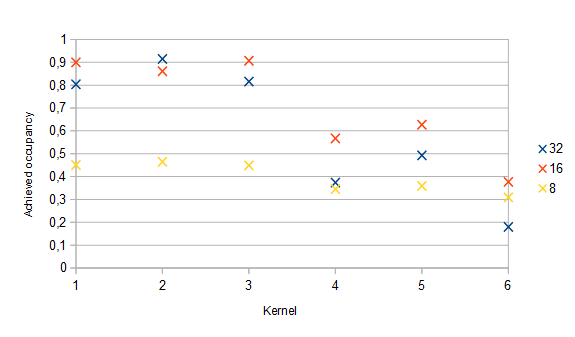
\includegraphics[width=0.85\textwidth]{fig/achievedoc_quadro.png}\label{fig:occupancy-quadro}
	\caption{Achieved occupancy on Quadro K1000M (Kepler) for the global memory method. The numbers 1-6 enumerate the kernels, where 1 is the detectSurvivorsInit kernel, 2-5 are detectSurvivors kernels and 6 is the final detectDetections kernel.}
\end{figure}
\end{center}

There are several things to note here. The first is the low occupancy of the 8x8 configuration, which varies between 30.9\% and 46.5\%. This can actually be predicted from \ref{tab:capability-3050}, where maximum number of blocks per streaming multiprocessor for compute capability 3.0 is 16, but the maximum number of threads is 2048. This means, that to reach full or almost full occupancy, at least 128 threads per block are needed. In case of 8x8 configuration, there are only 64 threads and so the maximum of 50\% occupancy for such configuration can be reached.

On the other hand for the last 3 kernels the occupancy is lower for all 3 configurations anyway, because the number of surviving samples is lower than the maximum occupancy. Another thing to note is, that lower achieved occupancy doesn't always mean lower performance. Even though 8x8 configuration has the lowest occupancy, and for the first three kernels the difference is 40-50\%, it still performs slightly better than the 32x32 configuration. This is due to higher global memory throughput in case of 8x8 and 16x16 kernels, which is a result of better memory coalescing.

\subsection{Memory throughput}

As mentioned 

\begin{center}
\begin{figure}[h]
	\centering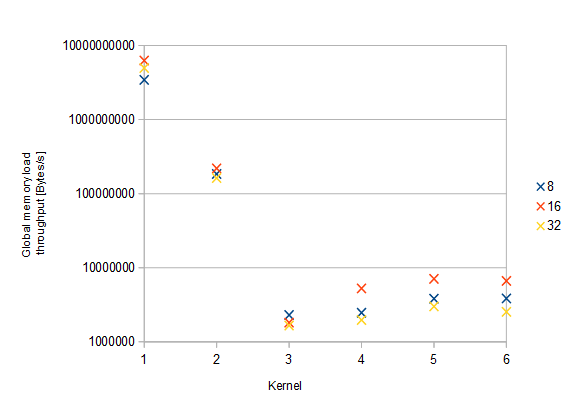
\includegraphics[width=0.85\textwidth]{fig/load_gthroughput_quadro.png}\label{fig:load-g-throughput}
	\caption{Load Global memory throughput on Quadro K1000M (Kepler) for the global memory method. The numbers 1-5 enumerate the kernels, where 1-4 are detectSurvivors kernels and 6 is the final detectDetections kernel.}
\end{figure}
\end{center}

\begin{center}
\begin{figure}[h]
	\centering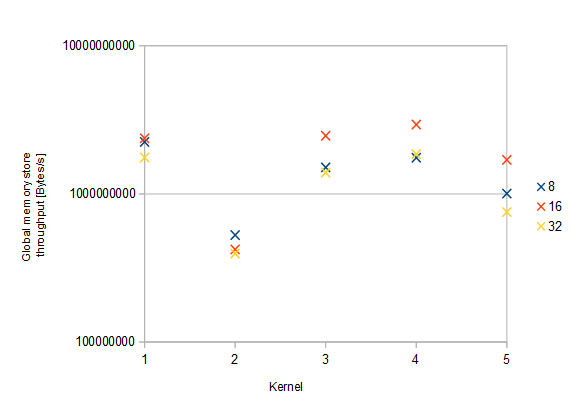
\includegraphics[width=0.85\textwidth]{fig/store_gthroughput_quadro.png}\label{fig:store-g-throughput}
	\caption{Achieved occupancy on Quadro K1000M (Kepler) for the global memory method. The numbers 1-6 enumerate the kernels, where 1 is the detectSurvivorsInit kernel, 2-5 are detectSurvivors kernels and 6 is the final detectDetections kernel.}
\end{figure}
\end{center}

\section{Summary}

As of \today ~the detector contains a working GPU and CPU implementations. The CPU version is available for comparison measurements and the GPU version is unoptimized with only a few GPU acceleration features. The latest version is available at: \url{https://github.com/mmaci/vutbr-fit-object-detection}.

\begin{itemize}
	\item Memory usage is likely to stay similar, as there aren't many more viable options. The only other option is unified memory in CUDA 6.0, which seems to be more of a programmer convenient, than performance feature and shared memory, which might be used for local optimizations.
	\item Bilinear interpolation using texture memory is used for image down-sampling, instead of a software implementation.
	\item LBP for 2x1, 1x2 and 2x2 features is calculated using texture memory bilinear interpolation, which leads to a speed-up due to the fact, that sum of the intensity values isn't needed and an average is used instead.
\end{itemize}

\section{Future work}

Some of the ideas and key features yet to be implemented are:

\begin{itemize}
	\item It is generally known, that most of the samples get discarded by the WaldBoost algorithm at the beginning as background. This leads to a large number of threads waiting for the few ones, that still compute. A measurement has to be taken to statistically determine the waiting-thread count and rearrange threads in a way to increase the percentage of running threads.
	\item Other methods of interpolation, such as Lanczos interpolation should be explored and measured compared to the current bilinear interpolation.
	\item The success rate and performance of the detector is also highly dependent on the pyramid image build, therefore other ways to build an optimized pyramid should be explored or if mipmaps can be used instead and thus the whole software based interpolation omitted.
	\item The CPU version should exactly match the algorithm used for the GPU version and also be optimized to provide a valid comparison.

\end{itemize}

%=========================================================================

\nocite{zemcik-high-performance}
\nocite{herout-realtime-cuda}